\documentclass{report}
\usepackage{hyperref}
\usepackage[ngerman]{babel}
\usepackage{amsmath}
\usepackage{amsfonts}
\usepackage{amsthm}
\usepackage{tcolorbox}
\usepackage[a4paper, total={7in, 9in}]{geometry}
\usepackage[font={scriptsize,it}]{caption}
\usepackage{scrextend}
\usepackage{graphicx}
\usepackage{caption}
\usepackage{subcaption}
\usepackage[utf8]{inputenc}
\usepackage[T1]{fontenc}
\DeclareUnicodeCharacter{2212}{-}
\usepackage{verbatim}
\usepackage{tikz}

\tikzset{
  treenode/.style = {shape=rectangle, rounded corners,
                     draw, align=center,
                     top color=white, bottom color=blue!20},
  root/.style     = {treenode, font=\Large, bottom color=red!30},
  env/.style      = {treenode, font=\ttfamily\normalsize},
  dummy/.style    = {circle,draw}
}

\tikzstyle{level 1}=[level distance=3.5cm, sibling distance=3.5cm]
\tikzstyle{level 2}=[level distance=3.5cm, sibling distance=2cm]

% floating figure for column
\newenvironment{Figure}
	{\par\medskip\noindent\minipage{\linewidth}}
	{\endminipage\par\medskip}

\begin{document}

\begin{titlepage}
   \vspace*{\stretch{1.0}}
   \begin{center}
      \Large\textbf{eHealth Lab09 - HS20}\\
      \large\textit{Results from Pascal Brunner - brunnpa7}
   \end{center}
   \vspace*{\stretch{2.0}}
\end{titlepage}

% Beispiel Bild
%\begin{Figure}
%   \centering
%    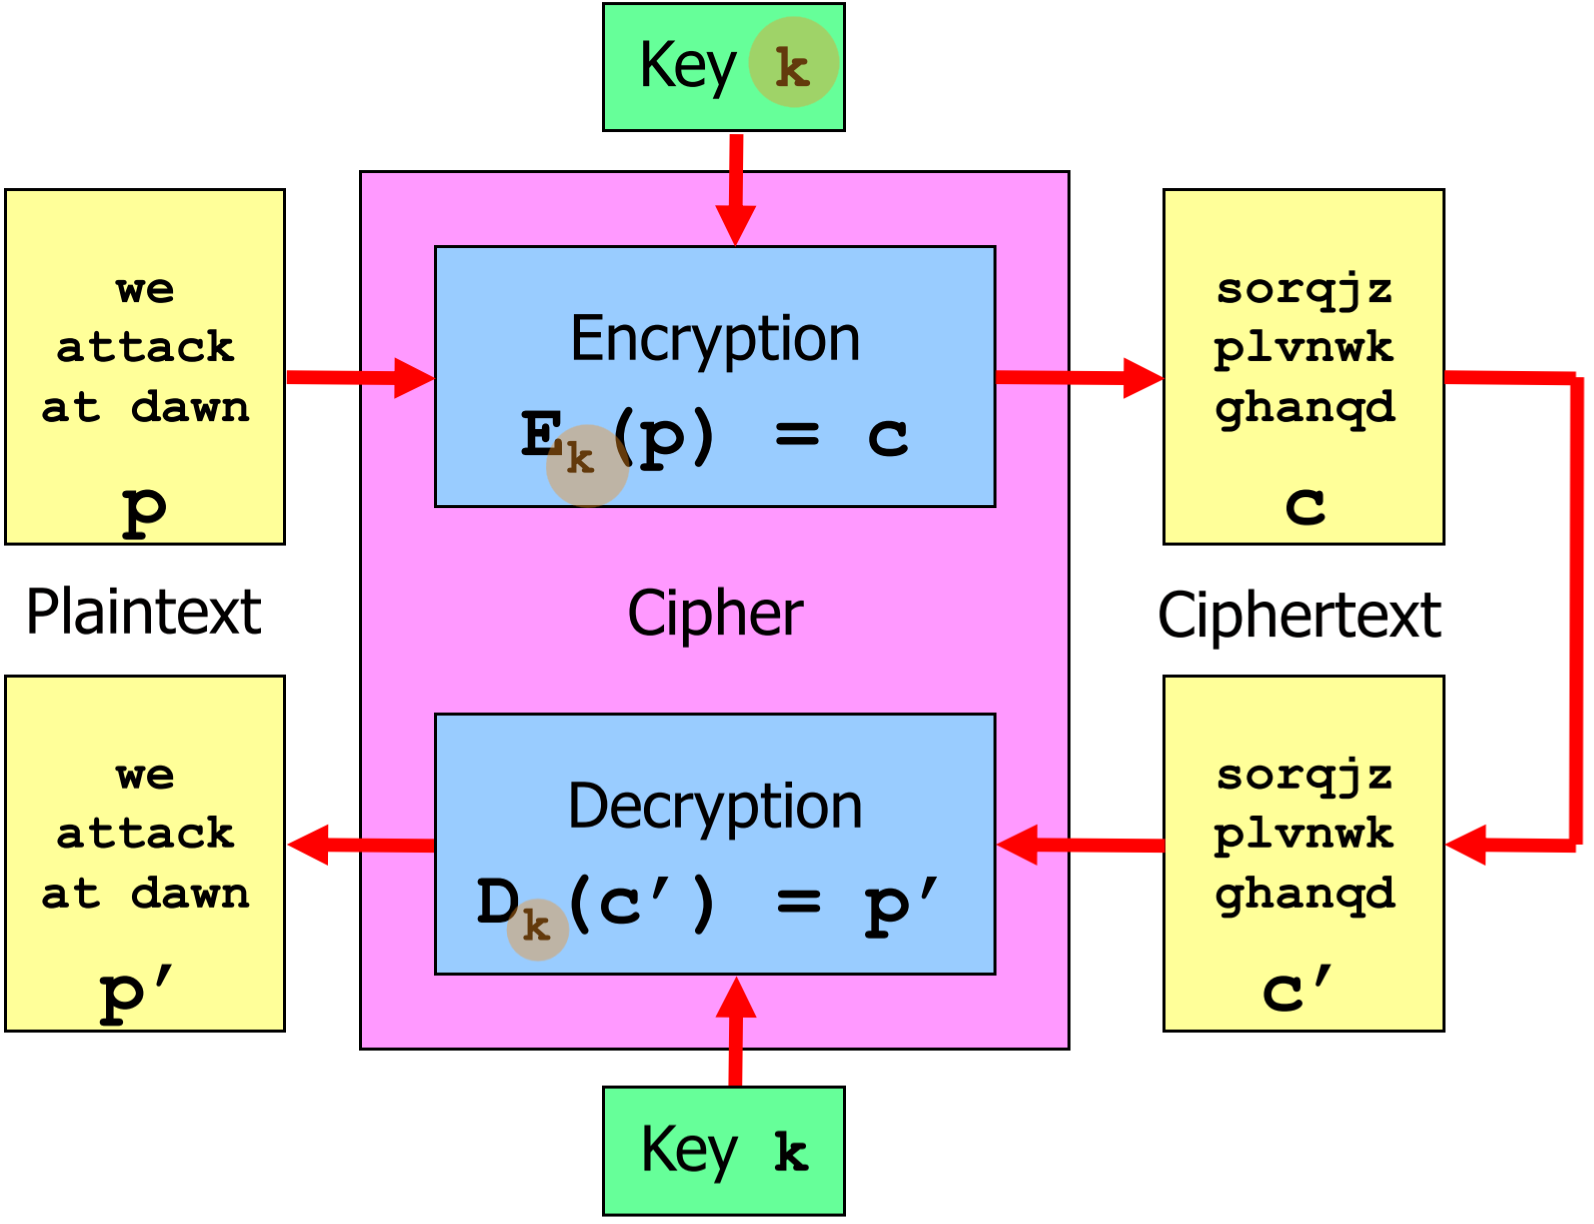
\includegraphics[width=150px]{img/BasicTerminologySecKeyCrypto.png}
%        \captionof{figure}{Basic Terminology basierend auf Secret Key Cryptography}
%        \label{fig:Basic Terminology}
%    \end{Figure}

\section*{Swiss Corona App}

The App has been developed in cooperation between Bundesamt für Information und Telekommunikation, ETH, EPFL as well as the Ubique. Ubique therefore has already developed a few swiss government apps such as SBB or MeteoSwiss.\\
One of the biggest challenges is to make sure that the valid 'social distance' is recognized within the app. E.g. If I stand with a distance of 5 meters to another person is this a invalid source to synchronize our IDs. But If I stand next to a person (let's say one meter)
our mobile phones should exchange the ID to make sure to notify the person if one of them is positiv tested.\\

Therefore is the main functionality to track the social distance between the different persons whereas it has to be synchronized if there is a chance that one person infect the other with the virus. This exchange happens with the technology 'Bluetooth'.
The app generated randomly the ID for a person, which is not trackable to a specific person, but to a mobile-phone user. Once there is an exchange between to person, the IDs are stored on the device for 14 days.
If a person is positiv tested to covid-19, they receive a code which they have to submit in the app. All person that might have been infected will be notified with a warning on the display.\\

There security is guaranteed since the data never leaves the mobile phones, furthermore the IDs are random generated and it is not possible to traceback who has met someone and at which time.\\

If we compare to all other apps we have installed on our mobile device with much more 'dangerours security settings', the swiss covid apps is a 'must-have' for every person in Switzerland. It is one of the easiest way to cut the chain-of-infection.
For me it's no questions to use the swiss-covid-App. If I meet a person who has not installed the app I am always curios why they haven't installed it. Mostly the have respect of the 'control of the government' or 'security-issues' 
During the discussion they realized, that Apps such as Whatsapp, facebook, instagram etc. have much more security-issues. I think the government or even other people should clarify the security-parts even with comparing to the most common apps


\end{document}